\chapter{Method}\label{method}
Chapter 4 will discuss the different methods utilised in the experiments and a rationale behind the methods. The chapter begins with an overview of the planned research plan and explains how the benchmark is developed. After that, various zero-cost proxies, such as \gls{FLOPs}, Params, EPE-NAS, L2-norm, Plain, Zen-score, and GradSign, are mathematically explained. Also, the implementation of the zero-cost proxies is provided. The chapter then looks into the combination of zero-cost proxies, discussing how to use the weighted arithmetic mean to combine proxies to rank architectures. Finally, the chapter evaluates the effectiveness of the different methods and techniques used in the study.

\section{Research Plan}
In this section, the research methods employed in this study are presented. As \cref{fig:research_flowchart} illustrates, the process comprises several steps. First, the process starts with generating random architectures, followed by comprehensive training of these architectures for benchmarking purposes. Subsequently, a zero-cost proxy framework is established, and data regarding the performance of zero-cost proxies is collected. Lastly, a quantitative analysis is conducted using the acquired data to conclude the performance and effectiveness of the zero-cost proxies. 
\clearpage

\begin{figure}[htbp]
\centering
\begin{tikzpicture}[
  node distance=1cm,
  process/.style={rectangle, rounded corners, minimum width=4cm, minimum height=1.5cm, text width=3.6cm, align=center, draw=black},
  process1/.style={process, fill=gray!20},
  process2/.style={process, fill=gray!50},
  arrow/.style={thick,->,>=stealth, line width=1.5pt, draw=gray}
]

\node (step1) [process1] {Generate Random Architectures};
\node (step2) [process2, below=of step1] {Conduct Comprehensive Training on Architectures for Benchmarking};
\node (step3) [process1, below=of step2] {Establish Zero-Cost Proxy Framework};
\node (step4) [process2, below=of step3] {Collect Data on Zero-Cost Proxies Performance};
\node (step5) [process1, below=of step4] {Perform Quantitative Analysis Using Collected Data};
% Add more nodes for additional steps

\draw [arrow] (step1) -- (step2);
\draw [arrow] (step2) -- (step3);
\draw [arrow] (step3) -- (step4);
\draw [arrow] (step4) -- (step5);
% Add more arrows for additional steps

\end{tikzpicture}
\caption{Flowchart illustrating the research process.}
\label{fig:research_flowchart}
\end{figure}

\section{Dataset}
\begin{comment}
Different datasets for \gls{HAR} had to be researched and justified to conduct experiments regarding the presented goal and research question. In this section, the chosen datasets will be presented with their workings and a justification for why it was appropriate for our experiments. 
\end{comment}

\Gls{ntu-rgbd} is a large-scale dataset for human activity analysis. It contains over 56 thousand video samples and 4 million frames. The NTU RGB+D dataset contains 60 action classes such as drinking, eating, staggering, punching and kicking \autocite{Shahroudy_2016_CVPR}. 

The dataset is collected using Microsoft Kinect v2 sensors, in which they collected four modalities: depth maps, 3D joint information, RGB frames and IR sequences. In total, 25 body joints were captured in the dataset, in which each body joint is represented by x-coordinates, y-coordinates and depth \autocite{Shahroudy_2016_CVPR}. The body joints are illustrated in \cref{fig:ntu_body_joints}. 

\begin{figure}[!ht]
    \centering
    \includegraphics[width=5cm]{figures/nturgb.drawio.png}
    \caption{1-base of the spine, 2-middle of the spine; 3-neck, 4-head, 5-left shoulder, 6-left elbow, 7-left wrist, 8-left hand, 9-right shoulder, 10-right elbow, 11-right wrist, 12-right hand, 13-left hip, 14-left knee, 15-left ankle, 16-left foot, 17-right hip, 18-right knee, 19-right ankle, 20-right foot, 21-spine, 22-tip of the left hand, 23-left thumb, 24-tip of the right hand, 25-right thumb}
    \label{fig:ntu_body_joints}
\end{figure}

The NTU RGB+D dataset was later expanded into a new one named NTU RGB+D 120. The new dataset contains 114 480 video samples of 120 action classes, all from 106 separate human subjects. 

The NTU RGB+D dataset has been employed in numerous studies, making it a well-established choice for research in the field of HAR \autocite{yan2018spatial, si2019attention, cheng2020skeleton}. The dataset's large scale and diverse range of activities facilitate the training of models with high generalisation capabilities, which aligns with the goals of this study in achieving optimal final validation accuracy. Given the dataset's widespread application and success in HAR-related research, it is an appropriate foundation for this investigation.
\section{Benchmark}
Within NAS, a benchmark is a collection of already trained and evaluated models that can be queried to obtain their validation accuracy. For research within NAS, such benchmarks are crucial as they spare the researchers thousands of GPU training time. Popular benchmarks within the literature are NAS-Bench-101 \autocite{ying2019bench}, NAS-Bench-201 \autocite{dong2020bench} and NAS-Bench-360 \autocite{tu2021bench}. These benchmarks contain thousand of trained and evaluated models on different datasets. However, to the best of our knowledge, 
there exist no similar benchmarks for GCN within HAR. Consequently, a benchmark had to be created for later experiments in the thesis. \Cref{sec:gcn-nas} highlights how the framework used for generating and training models works in detail, \cref{sec:full_trained} goes into how the authors define a fully trained model and \cref{subsec:experimentalsetup} explains the basic methodology behind the creation of the benchmark.       

\subsection{GCN-NAS}\label{sec:gcn-nas}
To create the benchmark, the authors used the framework in the paper Learning Graph Convolutional Network for Skeleton-Based Human Action Recognition by Neural Searching \autocite{peng2020learning}. The framework provides ways to train individual models and run the provided NAS algorithm to find the best architectures for a given problem. In addition, the framework is developed to be used on the NTU RGB+D dataset.  

The search space consists of eight function modules that can be applied in each network layer. To extract features $U$ from a given node in a graph, the filter $g_{\theta}$ is approximated using Chebyshev polynomials with R-th order. The more significant R, the bigger the local receptive field of the GCN layer will be. Chebyshev polynomial is recursive and is given in \cref{eq:chebyshev}. 

\begin{equation}
    \bm{Y} = \sum^R_{r=0} \theta_r' \bm{T_r} (\bm{\hat{L}})\bm{X},
    \label{eq:chebyshev}
\end{equation}

In which $ \theta_r'$ is the Chebyshev coefficient. Recursively, the Chebyshev polynomial $T_r(\hat{L})$ is defined by \cref{eq:cheb}. 

\begin{equation}
    \bm{T_r}(\bm{\hat{L}}) = 2 \bm{\hat{L}}\bm{T_{r-1}} (\bm{\hat{L}}) - \bm{T_{r-2}}(\bm{\hat{L}}),
    \label{eq:cheb}
\end{equation}

where $T_0$ = 1 and $t_1 = \hat{L}$. In the framework, $\hat{L}$ is normalised to the range $[-1,1]$, where $\hat{L} = \frac{2L}{\lambda_{max}} - I_n$. Based on the work of \autocite{DBLP:journals/corr/KipfW16}, $R = 1$ and $\lambda_{max} = 2$. This results in a first-order approximation of spectral graph convolutions, as shown in \cref{eq:shared}. 


\begin{equation}
\begin{aligned}
    \bm{Y} &= \theta'_0 \bm{X} + \theta'_1 (\bm{L} + \bm{I_n})\bm{X} \\
    &= \theta'_0 \bm{X} - \theta'_1(\bm{D}^{-\frac{1}{2}}\bm{A}\bm{D}^{-\frac{1}{2}})\bm{X}
\end{aligned}
\label{eq:shared}
\end{equation}

Similarly, $\theta^{'}$ can be approximated with a unified parameter $\theta$; this means that instead of using a separate parameter for $\theta^{'}$, it can be estimated using a single parameter, $\theta$, which will be a simplified representation of $\theta^{'}$. Then, Y is given by \cref{eq:y_final}. 

\begin{equation*}
\bm{Y} = \theta (\bm{I_n} + \bm{D}^{-\frac{1}{2}}\bm{A}\bm{D}^{-\frac{1}{2}})\bm{X}
\label{eq:y_final}
\end{equation*}

Given the available search space, the networks may have different combinations of R-th order Chebyshev-polynomials. Intuitively, using higher R-th order, the filters of each layer will be able to aggregate more information from the neighbours as the hops increase. 

In addition, the search space consists of three dynamic graph modules; spatial, temporal and spatial-temporal. Spatial features refer to the composition of the joints in a single frame, typically represented as a set of 3D coordinates. These spatial features capture the posture and pose of the human body at a given time point, but they do not capture the motion dynamics over time. On the other hand, temporal features capture how spatial features change over time. Through a series of frames, these features encode movement and action information. Finally, spatial-temporal features combine the spatial and temporal aspects to capture both the posture and dynamics of motion over time.  

To illustrate, \cref{fig:found_architecture} shows the best-performing architecture searched in the paper. 
\clearpage

\begin{table}[h!]
\centering
\caption{The searched architecture in the paper}
\begin{tabular}{lllllllll}
\hline
M & $L$ & $L^4_n$ & $L^4$ & $L^3$ & $L^2$ & $M(S)$ & $M(T)$ & $M(ST)$ \\ \hline
\multicolumn{1}{l|}{\cellcolor{verylightgray}{$k_1$}} & {\cellcolor{verylightgray}} &{\cellcolor{verylightgray}} &{\cellcolor{verylightgray}} &{\cellcolor{verylightgray}} & {\cellcolor{verylightgray}\checkmark} & {\cellcolor{verylightgray}\checkmark} & {\cellcolor{verylightgray}\checkmark} & {\cellcolor{verylightgray}\checkmark} \\
\multicolumn{1}{l|}{$k_2$} & & & & & & \checkmark & \checkmark & \checkmark \\
\multicolumn{1}{l|}{\cellcolor{verylightgray}{$k_3$}} & {\cellcolor{verylightgray}} &{\cellcolor{verylightgray}} &{\cellcolor{verylightgray}} &{\cellcolor{verylightgray}} &{\cellcolor{verylightgray}} & {\cellcolor{verylightgray}\checkmark} & {\cellcolor{verylightgray}\checkmark} & {\cellcolor{verylightgray}\checkmark} \\
\multicolumn{1}{l|}{$k_4$} & & & & & & \checkmark & \checkmark & \checkmark \\
\multicolumn{1}{l|}{\cellcolor{verylightgray}{$k_5$}} & {\cellcolor{verylightgray}} &{\cellcolor{verylightgray}} &{\cellcolor{verylightgray}} &{\cellcolor{verylightgray}} & {\cellcolor{verylightgray}\checkmark} & {\cellcolor{verylightgray}\checkmark} & {\cellcolor{verylightgray}\checkmark} &{\cellcolor{verylightgray}} \\
\multicolumn{1}{l|}{\textbf{$k_6$}} & & & & & \checkmark & & \checkmark & \\
\multicolumn{1}{l|}{\cellcolor{verylightgray}{$k_7$}} &{\cellcolor{verylightgray}} & {\cellcolor{verylightgray}\checkmark} &{\cellcolor{verylightgray}} &{\cellcolor{verylightgray}} & {\cellcolor{verylightgray}\checkmark} & {\cellcolor{verylightgray}\checkmark} & {\cellcolor{verylightgray}\checkmark} & {\cellcolor{verylightgray}\checkmark} \\
\multicolumn{1}{l|}{$k_8$} & & & & & \checkmark & & \checkmark & \\
\multicolumn{1}{l|}{\cellcolor{verylightgray}{$k_9$}} &{\cellcolor{verylightgray}} &{\cellcolor{verylightgray}} &{\cellcolor{verylightgray}} &{\cellcolor{verylightgray}} & {\cellcolor{verylightgray}\checkmark} &{\cellcolor{verylightgray}} & {\cellcolor{verylightgray}\checkmark} & {\cellcolor{verylightgray}}\\
\multicolumn{1}{l|}{$k_{10}$} & & & & & & & \checkmark & \\ \hline
\end{tabular}
\label{fig:found_architecture}
\end{table}

\Cref{fig:found_architecture} illustrates that the different layers of the architecture prefer different mechanisms. For instance, the lower layers prefer all the dynamic modules, whereas the deeper layers prefer the temporal representation correlations \autocite{peng2020learning}. 

\subsection{Definition of Fully Trained Models}\label{sec:full_trained}

Defining what constitutes a fully trained model is essential in the benchmark development context. Due to time and hardware resource limitations, a balance must be struck between training the models for optimal duration and ensuring the process remains feasible within the given constraints. 

A threshold was determined based on the trade-offs between computational cost, training time and model performance. By setting this upper limit, it was possible to maintain a reasonable training duration while still allowing the models to reach a  satisfactory level of performance. In the paper that introduced the framework, the authors \autocite{peng2020learning} opted to conclude the training process at 70 epochs, a practice adopted in the thesis.

Although the imposed threshold may not guarantee that every model reaches its absolute peak performance, it ensures that each model is trained sufficiently to compare relative performances. Furthermore, this definition of "fully trained" facilitates the efficient generation and evaluation of many models, which is crucial for successful benchmark development.




\subsection{Experimental Setup and Benchmarking Methodology}\label{subsec:experimentalsetup}

The algorithm for generating and evaluating random architectures is described in \cref{alg:random_arch_gen_eval}. The benchmark consists of a large-scale dataset comprising a diverse set of fully trained architectures to facilitate a comprehensive investigation into the performance of zero-cost proxies.

To generate random architectures, the framework described in \cref{sec:gcn-nas} was utilised as a foundation for developing an algorithm that implements a unique structure generation process to prevent the creation of duplicate architectures. The algorithm was constrained to create models consisting of four, six, eight, or ten layers to ensure a diverse range of architectures and explore a more comprehensive search space. In addition, other constraints were imposed, such as requiring at least one spatial, temporal, or spatial-temporal function module for effective feature extraction from the data.


\begin{comment}
    
\begin{algorithm}
\caption{Random Architecture Generation and Evaluation}
\label{alg:random_arch_gen_eval}
\begin{algorithmic}[1]
\Require{$N$: number of architectures to generate}
\State Define constraints for layer count and function modules
\State Initialize $i \gets 0$
\While{$i < N$}
    \State Generate a random architecture $A_i$ within constraints
    \If{not exists($A_i$)}
        \State Train $A_i$ for up to 70 epochs
        \State Compute validation accuracy $V_i$ of $A_i$
        \State Store $A_i$ and $V_i$ in the benchmark dataset
        \State $i \gets i + 1$
    \EndIf
\EndWhile
\end{algorithmic}
\end{algorithm}
\end{comment}

\begin{algorithm}
\caption{Random Architecture Generation and Evaluation}
\label{alg:random_arch_gen_eval}
\begin{algorithmic}[1]
\Require{$N$: number of architectures to generate}
\State Define constraints for layer count and function modules
\State Initialize $i \gets 0$
\While{$i < N$}
    \State Generate a random architecture $A_i$ within constraints
    \While{exists($A_i$)}
        \State Generate a new random architecture $A_i$ within constraints
    \EndWhile
    \State Train $A_i$ for up to 70 epochs
    \State Compute validation accuracy $V_i$ of $A_i$
    \State Store $A_i$ and $V_i$ in the benchmark dataset
    \State $i \gets i + 1$
\EndWhile
\end{algorithmic}
\end{algorithm}


\clearpage
The following hyperparameters were used for the training process: 

\begin{table}[h]
\centering
\caption{Hyperparameters for the training}
\begin{tabular}{ll}
\textbf{Name}                           & \textbf{Value}   \\ \hline
\multicolumn{1}{l|}{weight decay}       & $0.006$          \\
\multicolumn{1}{l|}{\cellcolor{verylightgray}base learning rate} & \cellcolor{verylightgray}$0.1$              \\
\multicolumn{1}{l|}{step}               & ${[}30, 45, 60{]}$ \\
\multicolumn{1}{l|}{\cellcolor{verylightgray}batch size}         & \cellcolor{verylightgray}$40$               \\
\multicolumn{1}{l|}{test batch size}    & $20$               \\
\multicolumn{1}{l|}{\cellcolor{verylightgray}num. epochs}        & \cellcolor{verylightgray}$70$               \\
\multicolumn{1}{l|}{nesterov}           & true            
\end{tabular}
\end{table}

It should be noted that while previous work in this field has utilised significantly larger benchmark datasets, time and hardware constraints necessitated limiting the scope of this benchmark to produce baseline results.

To provide insight into the characteristics of the benchmark dataset, \cref{tab:benchmark_stats} displays the minimum, average, and maximum values for training time and validation accuracy. Additionally, the number of layers in each architecture is provided.

\begin{table}[h]
    \centering
    \caption{Benchmark Dataset Statistics}
    \begin{tabular}{lrrr}
        \textbf{Statistic} & \textbf{Minimum} & \textbf{Average} & \textbf{Maximum} \\ \hline
        Training time (hours) & 4.35 & 13.16 & 53.30 \\
        \cellcolor{verylightgray}Validation accuracy & \cellcolor{verylightgray}0.92 & \cellcolor{verylightgray}0.94 & \cellcolor{verylightgray}0.95 \\
    \end{tabular}
    \label{tab:benchmark_stats}
\end{table}



\section{Zero-Cost Proxies}\label{zcproxies}

This section aims to provide a comprehensive overview of the different zero-cost proxies implemented in the project and clarify their respective methodologies.


\subsection{EPE-NAS}
The main idea behind EPE-NAS is to assess how the network's gradients behave concerning the neural network's input. Thus, the need for training an entire network is eliminated \autocite{lopes2021epe}. 

A linear map is defined as $w_i = f(x_i)$, in which $x_i$ is a sample from a batch $X$. The linear map can be computed by \cref{eq:linear}. 

\begin{equation}
    J_i = \frac{\delta f(x_i)}{\delta x_i}
    \label{eq:linear}
\end{equation}

However, it is necessary to see how the network will behave through different data points from the dataset. Therefore, the Jacobian matrix $w_i$ for different data points, $f(x_i)$, is calculated:

\begin{equation}
J = \begin{pmatrix}
\frac{\delta f(x_1)}{\delta x_1} & \frac{\delta f(x_2)}{\delta x_2} & \dots & \frac{\delta f(x_N)}{\delta x_N} 
 \end{pmatrix}^T
\end{equation}

The Jacobian matrix shows how the output of the network changes based on the input. After that, the correlation between data points of the same class is calculated to say how the untrained network can model complex functions \autocite{lopes2021epe}. The correlations are then used to calculate the covariance matrix for each class in the dataset:

\begin{equation}
    C_{J_c} = (J - M_{J_c})(J-M_{J_c})^t
\end{equation}
, where $M_J$ is:

\begin{equation}
    (M_{J_c})_{i,j} = \frac{1}{N} \sum_{n \in {1,...,N}} J_{i,n}
\end{equation}

Then, the correlation matrix is calculated for each class:

\begin{equation}
    C_{J_c} = \frac{(C_{J_c})_{i,j}}{\sqrt{(C_{J_c})_{i,j} * (C_{J_c})_{j,j}}}
\end{equation}


Each class is individually evaluated by summing the logarithm of the absolute values of the correlation matrix elements plus a small value $k = 1 \times 10^{-5}$.

\begin{equation}
    E_c = 
    \begin{cases}
        \sum^N_{i=1} \sum^N_{j=1}\ log(|(\sum_{J_c})_{i,j}| + K), & \text{if}\ C \leq \tau \\ \\ 
        \frac{\sum^N_{i=1} \sum^N_{j=1}\ log(|(\sum_{J_c})_{i,j}| + K)}{||\sum_{J_c}||}, & \text{otherwise}
    \end{cases}
\end{equation}

The network's score can be calculated using the evaluations of the correlation matrices above: 

\begin{equation}
    s = 
    \begin{cases}
        \sum_{t=1}^C |e_t|, & \text{if}\ C \leq \tau \\ \\ 
        \frac{\sum_{t=e}^C \sum_{j=i+1}^C |e_i - e_j|}{||e||}, & \text{otherwise}
    \end{cases}
\end{equation}

$e$ is the vector with the scores of the correlation matrices. For example, in the original paper \autocite{lopes2021epe}, they found empirically that $\tau = 100$. 


\subsection{Fisher}
Initially introduced as a pruning method in \autocite{DBLP:journals/corr/abs-1801-05787}, Fisher aims to remove feature maps or parameters that do not significantly contribute to the model's overall performance. This is achieved by eliminating activation channels and their corresponding parameters, estimated to have a negligible impact on the loss \autocite{abdelfattah2021zero}.

\cite{DBLP:journals/corr/abs-1801-05787} employed \cref{eq:fisher} to calculate the network score. 

\begin{equation}
    \centering
    S_z(z) = \left(\frac{\partial L}{\partial z}z\right)^2, S_n = \sum_{i=1}^M S_z(z_i)
    \label{eq:fisher}
\end{equation}

where $M$ is the length of the vectorised feature map, and  $S_z$ is the saliency per activation $z$. 

By mapping all the different layers of the network, the activations can be captured and used to score the network.  

\subsection{Flops}
% \glsreset{FLOPs}
As a zero-cost proxy, \Gls{FLOPs} is one of the simpler baselines as it simply goes through the model and calculates the number of floating point operations performed per second required to pass the input through the network. Therefore it could be considered a measure of the architecture's complexity \autocite{ning2021evaluating}. 

\subsection{Grad Norm}
The Gradient Norm is a straightforward zero-cost proxy that computes the sum of the Euclidean norms of gradients after conducting a single forward and backward pass using a minibatch of training data \autocite{abdelfattah2021zero}. Given a vector of gradients \(G = [g_1, g_2, ..., g_n]\), the gradient norm is calculated according to the formula presented in \cref{eq:gradnorm}.

\begin{equation}\label{eq:gradnorm}
    s = \sum_{i=1}^n \sqrt{g_i^2}
\end{equation}


\subsection{GradSign}
GradSign uses the network's initial gradients like many other zero-cost proxies do. However, the proxy's central concept uses $\Psi$(psi) to examine the optimisation landscape of various networks at the level of specific training samples. Thus, GradSign differs from most other gradient-based methods because of its theoretical insights. Under plausible assumptions, these theoretical results show that a network with denser sample-wise local optima has lower training and generalisation losses.

The calculation of $\Psi$ is often considered computationally infeasible for modern networks. To tackle this issue, the authors propose GradSign, which approximates $\Psi$. This method takes as input a mini-batch of sample-wise gradients that are evaluated at a randomly initialised point. Using this input, the method produces statistical evidence strongly associated with the well-trained predictive performance of the network, as measured by its accuracy on the entire dataset \autocite{zhang2021gradsign}. 


\subsection{Grasp}
\glsreset{GRASP}
\gls{GRASP} is one of the pruning-at-initialisation techniques. \cite{wang2020picking} argue that efficient training depends on preserving the gradient flow, from which the name gradient signal preservation comes. Therefore, \gls{GRASP} aims at finding the sub-networks as initialisation rather than after training. This is done by pruning the weights whose removal will cause a minor fall in the gradient norm after pruning \autocite{wang2020picking}. 


\subsection{Jacov}
The Jacov-score is a zero-cost proxy that estimates architecture performance by analysing the gradient correlation structure in a neural network's output space \autocite{jacob_conv}. The Jacov-score is computed using the eigenvalues of the correlation matrix of the batch Jacobian, as shown in \cref{eq:jacov}. 

\begin{equation}
    s =-\sum_i \left( \log(v_i+k)+\frac{1}{v_i+k}\right)
\label{eq:jacov}
\end{equation}

where $k$ is a small constant. The Jacov-score offers an efficient performance evaluation in \gls{NAS} without extensive computation.

\subsection{L2-norm}
L2-norm is calculated by summing over the norm of all weights of each layer in a neural network. 


\subsection{NAS-WOT}

\cite{jacob_conv} derived a metric by investigating linear maps of binary activation codes from the overlapping ReLU present at initialisation. These linear maps provide insight into how the network divides the input space.

The intuition is that the more similar the binary codes associated with two inputs are, the more challenging it is for the network to learn to separate them. When two inputs have the same binary code, they lie within the same linear region of the network and are particularly difficult to disentangle \autocite{jacob_conv}.

Let's consider a mini-batch of data $X = \{x_i\}^N_{i=1}$ mapped through a neural network as $f(x_ii)$. We can define an indicator variable $c_i$, forming a binary code defining a linear region. Using the binary codes, we can use Hamming distance $d_H(c_i, c_j)$ to measure how different the two inputs are \autocite{jacob_conv}.

The correspondence between binary codes in the mini-batch can be computed with the kernel matrix, as given in \cref{eq:naswot}.

\begin{equation} 
K_H = \begin{bmatrix} 
        N_A-d_H(c_1, c_1) & \dots & N_A-d_H(c_1, c_N) \\ 
        \vdots & \ddots & \vdots \\ 
        N_A-d_H(c_N, c_1) & \dots & N_A-d_H(c_N, c_N)
    \end{bmatrix}, 
    \label{eq:naswot}
\end{equation}
where $N_A$ is the number of ReLU activations in the network. Then the final score metric $s$ is derived from the logarithm of the kernel norm at initialisation. 

\begin{equation}
s = |log|K_H||
\end{equation}


Because of matrix instability, a small epsilon was added to the diagonal to make it possible to calculate a determinant.


\subsection{Params}
Within a neural network, there exist several trainable parameters, which, similarly to \gls{FLOPs}, are considered a measure of the architecture's complexity \autocite{ning2021evaluating}. 

\subsection{Plain}
The Plain-score is simply looping through all layers of the network. If the layer's weight contains a gradient, the gradient is multiplied by the layer's weights. Ultimately, the method is summing the scores to obtain the final score. 

\subsection{Snip}
\glsreset{SNIP}
The \gls{SNIP} method was introduced by \autocite{lee2018snip} as a pruning-at-initialisation technique, aiming to reduce the number of parameters within a neural network without affecting the accuracy during inference \autocite{frankle2020pruning}. \cite{frankle2020pruning} proposed a data-dependent saliency criterion that identifies significant connections in the network related to the current task before training. This approach enables the pruning of redundant connections, thus reducing the neural network's parameter count. The connections are identified based on their influence on the loss function.

\noindent In the paper Zero-Cost Proxies for Lightweight \gls{NAS} \autocite{abdelfattah2021zero}, \gls{SNIP} was repurposed as a zero-cost proxy. The score of the neural network was obtained by summing all parameters $N$ in the model according to \cref{eq:sumsnip},

\begin{equation}\label{eq:sumsnip}
S_n = \sum_{i=1}^N S_p(\theta)_i
\end{equation}

\begin{equation}
S_p(\theta) = \left|\frac{\partial L}{\partial \theta} \odot \theta\right|
\end{equation}

where $L$ is the loss function, \(\theta \) represents the parameters of the neural network, and \(\odot\) denotes the Hadamard product.



\subsection{Synflow}
\glsreset{Synflow}
\gls{Synflow}, originally proposed in \autocite{tanaka2020pruning}, is a method for parameter pruning. By pruning less significant parameters, highly sparse networks can be obtained with reduced network size while maintaining similar accuracy. \gls{Synflow} is built on three main principles: avoiding layer collapse, conservation of synaptic saliency, and magnitude pruning.

\noindent Layer collapse occurs when an algorithm prunes all parameters in a single weight layer, even when prunable parameters remain elsewhere in the network. This makes the network untrainable, as evidenced by sudden drops in achievable accuracy \autocite{tanaka2020pruning}. Therefore, it is crucial to avoid layer collapse since the network will become unusable if a layer is removed.

\noindent Synaptic saliency is a class of score metrics that can be expressed as the Hadamard product (\cref{eq:hadamardproduct}).

\begin{equation}
S(\theta) = \frac{\partial R}{\partial \theta} \odot \theta
\label{eq:hadamardproduct}
\end{equation}
where $R$ is a scalar loss function of the output $y$ of a feed-forward network parameterized by $\theta$ \autocite{tanaka2020pruning}. The conservation of synaptic saliency theorem demonstrates that the sum of synaptic saliency for all incoming parameters to a hidden neuron equals the sum of the synaptic saliency for the outgoing parameters from the hidden neuron \autocite{tanaka2020pruning}. Consequently, the sum of synaptic saliency for all incoming parameters to a hidden layer equals the sum of the synaptic saliency for the outgoing parameters from the hidden layer. This can lead to issues when performing one-shot pruning, where a larger layer would have parameters with lower synaptic saliency. In comparison, a smaller layer would have parameters with higher synaptic saliency. Pruning one of the parameters for a smaller layer would result in pruning almost all the parameters in a larger layer to compensate for the conservation of synaptic saliency, leading to layer collapse.

\noindent To prevent this, \gls{Synflow} introduces iterative pruning (magnitude pruning) by recalculating the synaptic saliency for all parameters at each iteration. This re-evaluation process gives new scores to parameters with lower scores in previous iterations, eliminating the imbalance between smaller and larger layers and reducing the possibility of layer collapse.
\noindent The \gls{Synflow} algorithm is described in \cref{eq:synflowalg}:

\begin{equation}\label{eq:synflowalg}
R_{SF} = \mathbbm{1}^T \left( \prod^L_{l=1} |\theta^{[l]}| \right) \mathbbm{1}
\end{equation}

The algorithm takes an input of ones (e.g., an image where all the pixels have the value 1) and performs a forward pass through the network. The loss $R$ is obtained by calculating the product of the output. This loss is then backpropagated through the network to the layers, and \cref{eq:hadamardproduct} is used to compute the synaptic saliency score for each parameter $\theta$.


\subsection{Zen-score}
Zen-score is a measure of the expressivity of the network, which is computationally efficient and correlates positively with the model accuracy \autocite{lin2021zen}. Zen-score builds upon the expected Gaussian complexity ($\Phi$-score), which can define the expressivity of a \Gls{VCNN}. In theoretical investigations, \gls{VCNN} is a frequently used prototype in which several convolutional layers are stacked to form the main body of the network. Each layer has a convolutional operator followed by a ReLU activation function, where residual links and Batch Normalisation are excluded. A global average pool layer (GAP) brings the feature map resolution down to 1 x 1 before a fully-connected layer  \autocite{lin2021zen}.  

However, numerical overflow may occur for deep networks when directly calculating the $\Phi$-score because of gradient explosion without batch normalisation layers \autocite{lin2021zen}. Zen-Score addresses this problem by adding batch normalisation layers and re-scaling the $\Phi$-score by some constant. 

\subsection{Summary}

\Cref{tab:summary_zc} displays an overall view of the discussed zero-cost proxies, with the characteristics of each method's data dependence, data independence and type outlined. 

\begin{table}[htbp]
\centering
{\footnotesize
\caption{Summary of the implemented zero-cost proxies in the project}
\begin{tabular}{lccc}
\textbf{Zero-Cost Proxy} & \textbf{Data-dependent} & \textbf{Data-independent} & \textbf{Type} \\ \hline
\multicolumn{1}{l|}{\cellcolor{verylightgray}Epe-NAS} & \checkmark \cellcolor{verylightgray} & \cellcolor{verylightgray} & \cellcolor{verylightgray} Jacobian  \\
\multicolumn{1}{l|}{Fisher} & \checkmark  &  & Pruning-at-init  \\
\multicolumn{1}{l|}{\cellcolor{verylightgray}Flops} & \cellcolor{verylightgray} \checkmark & \cellcolor{verylightgray} & \cellcolor{verylightgray} Baseline \\
\multicolumn{1}{l|}{GradNorm} & \checkmark &  & Pruning-at-init  \\
\multicolumn{1}{l|}{\cellcolor{verylightgray}GradSign} & \cellcolor{verylightgray} \checkmark & \cellcolor{verylightgray} & \cellcolor{verylightgray} Gradient Sign \\
\multicolumn{1}{l|}{Grasp} & \checkmark  &  & Pruning-at-init  \\
\multicolumn{1}{l|}{\cellcolor{verylightgray}Jacov} & \cellcolor{verylightgray} \checkmark & \cellcolor{verylightgray} & \cellcolor{verylightgray} Jacobian \\
\multicolumn{1}{l|}{L2-norm} &  & \checkmark  & Baseline  \\
\multicolumn{1}{l|}{\cellcolor{verylightgray}Nwot} & \cellcolor{verylightgray} \checkmark & \cellcolor{verylightgray} & \cellcolor{verylightgray} Jacobian \\
\multicolumn{1}{l|}{Params} &  & \checkmark  & Baseline  \\
\multicolumn{1}{l|}{\cellcolor{verylightgray}Plain} & \cellcolor{verylightgray} \checkmark & \cellcolor{verylightgray} & \cellcolor{verylightgray} Baseline \\
\multicolumn{1}{l|}{Snip} & \checkmark  &  & Pruning-at-init \\
\multicolumn{1}{l|}{\cellcolor{verylightgray}Synflow} & \cellcolor{verylightgray} & \cellcolor{verylightgray} \checkmark & \cellcolor{verylightgray} Pruning-at-init \\
\multicolumn{1}{l|}{Zen} &  &  \checkmark & Piece. Lin.  \\
\end{tabular}
\label{tab:summary_zc}
}
\end{table}





\section{Zero-Cost Framework}\label{sec:zc-framework}

A novel Zero-Cost framework was created to calculate the scores of each zero-cost proxy. The framework, influenced by \cref{abdelfattah}, has been developed as a versatile plug-and-play solution easily integrated into any \gls{NAS} project. The primary goal of this framework is to provide an efficient and effective means of using zero-cost proxies for performance prediction. These proxies are described in detail in \cref{zcproxies}.

\begin{algorithm}
    \begin{algorithmic}[1]
        \caption{Calcuate Zero-Cost Proxies}\label{alg:zc_framework}
        \Require model, dataLoader, lossFunction, override
        \State scoreStore $\gets$ Initialise store
        \State proxies $\gets$ getProxies() \Comment{Get all implemented proxies}
        \\
        \For{proxy in proxies}
            \If{override is not empty}
                \If{proxy not in override}
                    \State skip
                \EndIf
            \EndIf
            \\
            \State startTime $\gets$ now()
            \State score $\gets$ proxy.calculateProxy(model, dataLoader, lossFunction)
            \State scoreStore.proxy.time $\gets$ $\text{now()}-\text{startTime}$
            \State scoreStore.proxy.score $\gets$ score
        \EndFor
        \\
        \State \Return scoreStore
        
    \end{algorithmic}
\end{algorithm}

\Cref{alg:zc_framework} outlines calculating Zero-Cost proxies for a given model. The algorithm takes four inputs: the model, a data loader, a loss function, and an optional override parameter. The model represents the neural network architecture under evaluation, while the data loader and the loss function are used for calculating the proxy metrics. The optional override parameter allows users to calculate only specified proxies selectively.

An empty \textit{scoreStore} is initialised to keep track of the calculated scores and the time taken for each proxy. The algorithm then retrieves all the available proxy implementations using the \textit{getProxies()} function. Next, a loop iterates through each proxy, and if the optional override parameter is not empty, it checks whether the current proxy is included in the override list. If the proxy is not in the list, it is skipped, and the loop continues to the next proxy.

For each selected proxy, the algorithm records the start time. Then, it calculates the proxy score using the \textit{calculateProxy()} function with the model, data loader, and loss function as inputs. After calculating the score, the algorithm computes the time taken by subtracting the start time from the current time. Each proxy's calculated score and time are stored in the \textit{scoreStore}.

\begin{comment}
    
Finally, the \textit{scoreStore} containing scores and computation times for all the calculated proxies is returned. This information can be utilised by \gls{NAS} projects to predict the performance of various architectures efficiently without the need for expensive training or evaluation processes. In addition, the plug-and-play nature of the framework allows researchers and developers to easily integrate it into their projects, making performance prediction more accessible and reliable.
\end{comment}
\section{Correlation}\label{sec:corr}

Calculating the correlation between the score each zero-cost proxy provides and the validation accuracy is a logical approach to understanding the impact of the zero-cost proxies. Spearman Rank Correlation is a non-parametric statistical test that measures the strength and direction of the association between two ranked variables \autocite{hauke2011comparison}. The Spearman Rank does not assume a linear relationship between the two variables. It is suitable for cases where the connection between the validation accuracy and the zero-cost proxy may not be linear because it establishes the strength of a monotonic relationship. Additionally, the metric is less vulnerable to outliers because it focuses on the rank of the variables rather than their raw values.

Exploring other correlation measures, such as the Pearson correlation coefficient, provides additional perspective. Pearson's is the most commonly used correlation method and provides insights into the strength and direction of a linear relationship \autocite{turney2022pearson}. 

However, its utility for our project is limited due to several constraints. First, it assumes the variables in the dataset are normally distributed \autocite{turney2022pearson}. The Shapiro-Wilk test is a statistical test used to check whether a sample of numbers has been drawn from a normally distributed population, such that the null hypothesis is that the population is normally distributed \autocite{shaphiro1965analysis}. The null hypothesis is disregarded if the test's calculated p-value is less than the predetermined alpha level, typically 0.05. Discarding the null hypothesis means we have enough evidence to conclude that the data set under investigation does not exhibit a normal distribution. The Shapiro-Wilk test result for each variable (zero-cost proxy) is shown in \cref{tab:p_values}. 

\begin{table}[h]
\caption{P-values for each variable using the Shapiro-Wilk test}
\centering
\begin{tabular}{lr}
\textbf{Name} & \textbf{P-value} \\ \hline
\multicolumn{1}{l|}{\cellcolor{verylightgray}epe\_nas} & \cellcolor{verylightgray}$<1e-6$ \\
\multicolumn{1}{l|}{fisher} & $< 1e-6$ \\
\multicolumn{1}{l|}{\cellcolor{verylightgray}flops} & \cellcolor{verylightgray} $< 1e-6$ \\
\multicolumn{1}{l|}{grad\_norm} & $< 1e-6$ \\
\multicolumn{1}{l|}{\cellcolor{verylightgray}grad\_sign} & \cellcolor{verylightgray}$< 1e-6$ \\
\multicolumn{1}{l|}{grasp} & $< 1e-6$ \\
\multicolumn{1}{l|}{\cellcolor{verylightgray}jacov} & \cellcolor{verylightgray}$< 1e-6$ \\
\multicolumn{1}{l|}{l2\_norm} & $< 1e-6$ \\
\multicolumn{1}{l|}{\cellcolor{verylightgray}nwot} & \cellcolor{verylightgray}$0.003$ \\
\multicolumn{1}{l|}{params} & $< 1e-6$ \\
\multicolumn{1}{l|}{\cellcolor{verylightgray}plain} & \cellcolor{verylightgray} $< 1e-6$ \\
\multicolumn{1}{l|}{snip} & $< 1e-6$ \\
\multicolumn{1}{l|}{\cellcolor{verylightgray}synflow} & \cellcolor{verylightgray}$< 1e-6$ \\
\multicolumn{1}{l|}{val\_acc} & $< 1e-6$ \\
\multicolumn{1}{l|}{zen} & $< 1e-6$ \\
\end{tabular}
\label{tab:p_values}
\end{table}

The p-values for all variables are smaller than the significance level ($\alpha = 0.05$), as seen in the \cref{tab:p_values}. Therefore, we can disprove the Shapiro-Wilk test's null hypothesis for each variable, showing that the distributions of those variables considerably deviate from the normal distribution.

Further, Pearson's correlation is highly sensitive to outliers. A few extreme observations can greatly distort the correlation coefficient, potentially leading to incorrect interpretations. This sensitivity is unwanted given that the zero-cost proxies may contain such outliers, as illustrated in \cref{fig:zero_cost_proxies_outliers}, in which one can observe that the data contains outliers. 

Lastly, the Pearson correlation coefficient relies on the actual values of the variables, whereas our focus is more on their rankings, which makes the Spearman rank correlation a more suitable measure for our project.


\clearpage

\begin{figure}[h!]
  \centering
    \begin{adjustbox}{width=1.2\columnwidth,center}
  \begin{tabular}{ccc}
    \includesvg[width=0.5\textwidth]{figures/zc-proxies/epe_nas.svg} &
    \includesvg[width=0.5\textwidth]{figures/zc-proxies/fisher.svg} &
    \includesvg[width=0.5\textwidth]{figures/zc-proxies/flops.svg} \\
    \includesvg[width=0.5\textwidth]{figures/zc-proxies/grad_norm.svg} &
    \includesvg[width=0.5\textwidth]{figures/zc-proxies/grad_sign.svg} &
    \includesvg[width=0.5\textwidth]{figures/zc-proxies/grasp.svg} \\
    \includesvg[width=0.5\textwidth]{figures/zc-proxies/jacov.svg} &
    \includesvg[width=0.5\textwidth]{figures/zc-proxies/l2_norm.svg} &
    \includesvg[width=0.5\textwidth]{figures/zc-proxies/nwot.svg} \\
    \includesvg[width=0.5\textwidth]{figures/zc-proxies/params.svg} &
    \includesvg[width=0.5\textwidth]{figures/zc-proxies/plain.svg} &
    \includesvg[width=0.5\textwidth]{figures/zc-proxies/snip.svg} \\
    \includesvg[width=0.5\textwidth]{figures/zc-proxies/synflow.svg} &
    \includesvg[width=0.5\textwidth]{figures/zc-proxies/zen.svg} 
  \end{tabular}
  \end{adjustbox}
  \caption{Each zero-cost proxy normalised with the validation accuracy}
  \label{fig:zero_cost_proxies_outliers}
\end{figure}

The Spearman Rank Correlation is denoted by the symbol $\rho$ (rho) and ranges from -1 to 1, where -1 indicates a perfect negative relationship, 1 indicates a perfect positive relationship, and 0 shows no connection, as illustrated in \cref{fig:correlations_illustrated} \autocite{laerdstatistics}.  

\begin{figure}[h]
\centering
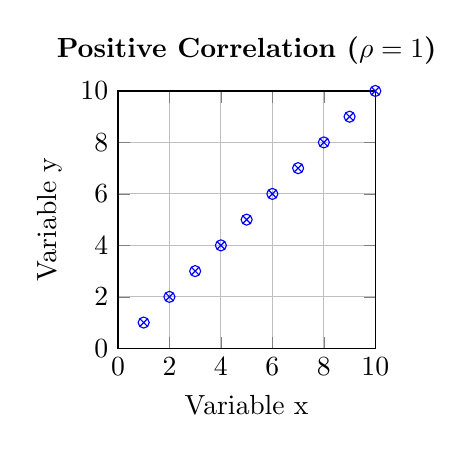
\begin{tikzpicture}
\begin{axis}[
    title={\textbf{Positive Correlation ($\rho = 1$)}},
    xlabel={Variable x},
    ylabel={Variable y},
    xmin=0, xmax=10,
    ymin=0, ymax=10,
    xtick={0,2,4,6,8,10},
    ytick={0,2,4,6,8,10},
    grid=major,
    legend pos=south east,
    width=0.4\textwidth,
    height=0.4\textwidth,
]
\addplot[
    only marks,
    mark=otimes,
    color=blue,
] coordinates {
(1,1)(2,2)(3,3)(4,4)(5,5)(6,6)(7,7)(8,8)(9,9)(10,10)
};
\end{axis}
\end{tikzpicture}
\hspace{1cm}
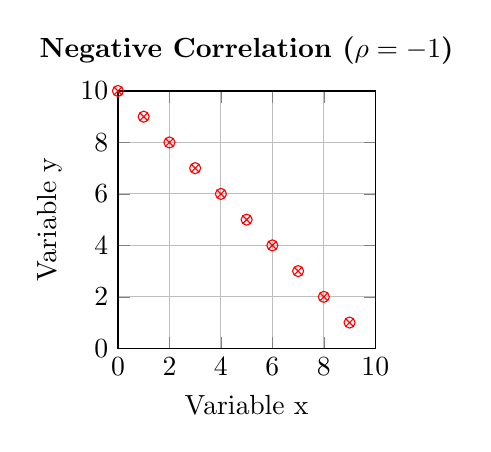
\begin{tikzpicture}
\begin{axis}[
    title={\textbf{Negative Correlation ($\rho = -1$)}},
    xlabel={Variable x},
    ylabel={Variable y},
    xmin=0, xmax=10,
    ymin=0, ymax=10,
    xtick={0,2,4,6,8,10},
    ytick={0,2,4,6,8,10},
    grid=major,
    legend pos=south east,
    width=0.4\textwidth,
    height=0.4\textwidth,
]
\addplot[
    only marks,
    mark=otimes,
    color=red,
] coordinates {
(9,1)(8,2)(7,3)(6,4)(5,5)(4,6)(3,7)(2,8)(1,9)(0,10)
};
\end{axis}
\end{tikzpicture}
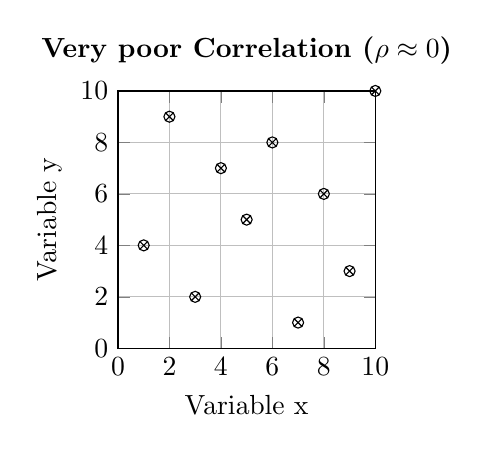
\begin{tikzpicture}
\begin{axis}[
    title={\textbf{Very poor Correlation ($\rho \approx 0$)}},
    xlabel={Variable x},
    ylabel={Variable y},
    xmin=0, xmax=10,
    ymin=0, ymax=10,
    xtick={0,2,4,6,8,10},
    ytick={0,2,4,6,8,10},
    grid=major,
    legend pos=south east,
    width=0.4\textwidth,
    height=0.4\textwidth,
]
\addplot[
    only marks,
    mark=otimes,
    color=black,
] coordinates {
(1,4)(2,9)(3,2)(4,7)(5,5)(6,8)(7,1)(8,6)(9,3)(10,10)
};
\end{axis}
\end{tikzpicture}

\caption{Scatter plots illustrating perfect positive, perfect negative correlations and very poor correlation}
\label{fig:correlations_illustrated}
\end{figure}

Spearman Rank Correlation works by calculating the difference in ranks of the two variables for each observation, then squaring these differences and summing them up, as given in \cref{eq:spearman}. 

\begin{equation} 
    \rho = 1 - \frac{6 \sum d_i^2}{n(n^2 - 1)}, 
    \label{eq:spearman}
 \end{equation}

where $d_i$ is the difference in ranks for each observation, and $n$ is the number of observations.

In the context of zero-cost proxies and validation accuracy, Spearman Rank Correlation can be used to determine whether there is a monotonic relationship between the two. A positive correlation would indicate that as the zero-cost proxy improves, so does the validation accuracy, while a negative correlation would imply an inverse relationship. A correlation near zero would suggest that the two variables have little or no association. 




\section{Exploration of Zero-Cost Proxies via Warmup Strategy}
\subsection{Theoretical and Practical Considerations}

\begin{comment}
    
The primary objective of \gls{NAS} is to discover high-performing architectures while minimising computational overhead. Training numerous architectures for a large number of epochs is computationally prohibitive. Training architectures for a limited number of epochs may be a more viable approach. In this context, we introduce the concept of a warmup strategy in this study, which aims to determine an optimal epoch threshold that can provide a reliable estimation of the relative performance of different architectures.
\end{comment}

In this section, we introduce the concept of a warmup strategy, which aims to determine an optimal epoch threshold that can provide a reliable estimation of the relative performance of different architectures. This contrast with the naive NAS approach of training numerous architectures, which can be computationally prohibitive. 

The underlying principle for this strategy is based on the assumption that training an architecture for $x$ epochs offers a more efficient evaluation than training the same architecture for $y$ epochs if $x < y$. By identifying an appropriate warmup threshold, researchers can effectively balance the trade-off between computational expense and the accuracy of architecture performance estimation.

To achieve this, each architecture is trained for a predetermined number of warmup epochs, and the zero-cost proxies are calculated at each epoch. Then, for every epoch, the Spearman Rank correlation coefficient between the zero-cost proxies and the final validation accuracy for all architectures is calculated. The epoch with the highest correlation is considered the optimal warmup point. 



\section{Combining Zero-Cost Proxies}

Upon analysing the outcomes derived from addressing research question 1 and research question 2, it became necessary to reconsider the experimental plan. The insights gained from the initial results prompted further exploration into utilising zero-cost proxies. Consequently, a decision was made to undertake additional ad hoc experiments to delve deeper into this area of investigation.



\subsection{Majority Vote Method}\label{subsec:vote}

The majority vote method, introduced by \cite{abdelfattah2021zero}, is an approach for ranking candidate architectures based on the pooled results of multiple zero-cost proxy metrics. This technique consolidates the rankings generated by different zero-cost proxy metrics, and the architectures are ranked according to the majority vote derived from these metrics. The algorithm of the voting method is outlined in \cref{alg:vote}. 

\begin{algorithm}[h!]
\caption{Voting Accuracy for Metric Combinations}\label{alg:vote}
\begin{algorithmic}[1]
\Function{vote}{$mets$, $gt$}
    \State $numpos \leftarrow 0$ \Comment{Initialize the number of positive elements}
    \For{each element $m$ in $mets$}
        \If{$m > 0$}
            \State Increment $numpos$ by 1
        \EndIf
    \EndFor
    \If{majority of elements in $mets$ are positive}
        \State $sign \leftarrow +1$
    \Else
        \State $sign \leftarrow -1$
    \EndIf
    \State \Return $sign * gt$ 
\EndFunction
\vspace{1em}
\Function{calc}{$acc$, $metrics$, $comb$}
    \State $num\_pts$ \Comment{Initialize the total number of data points }
    \State $tot \leftarrow 0$, $right \leftarrow 0$
    \For{each pair of distinct indices $i$ and $j$}
        \State $diff \leftarrow acc[i] - acc[j]$
        \If{$diff \neq 0$}
            \State $diffsyn$ \Comment{Initialize an empty list}
            \For{each metric $m$ in $comb$}
                \State $diffsyn \leftarrow metrics[m][i] - metrics[m][j]$
            \EndFor
            \State \textit{/* Check if $diffsyn$ and $diff$ have same sign */}
            \State $same\_sign \leftarrow$ \Call{vote}{$diffsyn$, $diff$}
            \If{$same\_sign > 0$}
                \State Increment $right$ 
            \EndIf
            \State Increment $tot$
        \EndIf
    \EndFor
    \State $votes \leftarrow \frac{right}{tot}$ \Comment{Calculate the voting accuracy}
    \State \Return $(comb, votes)$
\EndFunction
\end{algorithmic}
\end{algorithm}


Given that it is uncertain which combination of zero-cost proxies would yield the best results, the authors developed a function to generate all possible subsets of the 14 zero-cost proxy metrics. Subsequently, the majority vote for each subset was calculated and compared to the ground truth provided by the validation accuracy of every trained architecture in the benchmark. For example, \cref{tab:example_architectures} displays two architectures with given values for three zero-cost proxies (\gls{Synflow}, \gls{SNIP} and Grad Sign) and their validation accuracy. 

\begin{table}[h]
\centering
\caption{Example of two architectures with validation accuracy and zero-cost proxy metrics.}
\begin{tabular}{ll}
\textbf{Architecture} & \textbf{Metrics}          \\ \hline
\multicolumn{1}{l|}{1} & \multicolumn{1}{l}{Validation Accuracy: 0.85} \\
\multicolumn{1}{l|}{\cellcolor{verylightgray}} & \cellcolor{verylightgray}Synflow: 0.62 \\
\multicolumn{1}{l|}{} & \multicolumn{1}{l}{SNIP: 0.75} \\
\multicolumn{1}{l|}{\cellcolor{verylightgray}} & \cellcolor{verylightgray}Grad Sign: 0.28 \\ \hline
\multicolumn{1}{l|}{2} & \multicolumn{1}{l}{Validation Accuracy: 0.89} \\
\multicolumn{1}{l|}{\cellcolor{verylightgray}} & \cellcolor{verylightgray}Synflow: 0.48 \\
\multicolumn{1}{l|}{} & \multicolumn{1}{l}{SNIP: 0.82} \\
\multicolumn{1}{l|}{\cellcolor{verylightgray}} & \cellcolor{verylightgray}Grad Sign: 0.36
\end{tabular}
\label{tab:example_architectures}
\end{table}

By examining the validation accuracy, one can deduce that Architecture 2 is superior to Architecture 1. Upon analysing the computed zero-cost proxy metrics, the following observations can be made:

\begin{itemize}
\item \textbf{Synflow}: Architecture 1 $(0.62) >$ Architecture 2 $(0.48)$
\item \textbf{SNIP}: Architecture 1 $(0.75) <$ Architecture 2 $(0.82)$
\item \textbf{GradSign}: Architecture 1 $(0.28) <$ Architecture 2 $(0.36)$
\end{itemize}

In this case, one positive difference (\gls{Synflow}) and two negative differences (\gls{SNIP} and Grad Sign). Consequently, the majority vote favours Architecture 2, consistent with the validation accuracy.

\subsection{Weighted Arithmetic Mean}
The weighted arithmetic mean, as described in \autocite{wam}, is a widely used technique in statistics and data analysis. This study applied the weighted arithmetic mean method to the zero-cost proxies using Spearman's rank correlation as weights for ranking various architectures.

\begin{algorithm}
\caption{Weighted Arithmetic Mean for datapoint $d$}\label{alg:weighted_mean}
\begin{algorithmic}[1]
\Require Zero-cost proxies $P_d = \{p_1, p_2, \dots, p_n\}$
\Require Validation accuracy $A_d$
\State Normalise zero-cost proxies: $P_{d_{norm}} = \{p_{1_{norm}}, p_{2_{norm}}, \dots, p_{n_{norm}}\}$
\For{$i = 1$ to $n$}
    \State Calculate Spearman's rank correlation $r_i$ between $p_{i_{norm}}$ and $A_d$
    \State Assign weight $w_i = r_i$
\EndFor
\State Initialize: $\text{Score}_d \leftarrow 0$, $total\_weight \leftarrow 0$
\For{$i = 1$ to $n$}
    \State $\text{Score}_d \leftarrow \text{Score}_d + (p_{i_{norm}} * w_i)$
    \State $total\_weight \leftarrow total\_weight + w_i$
\EndFor
\State $\text{Score}_d \leftarrow \frac{\text{Score}_d}{total\_weight}$
\State Calculate correlation between $\text{Score}_d$ and $A_d$ using Spearman's rank correlation
\end{algorithmic}
\end{algorithm}


As illustrated in \cref{alg:weighted_mean}, each zero-cost proxy value is first normalised with min-max normalisation, ensuring they are on a comparable scale for accurate comparison and combination. Next, weights were assigned to each zero-cost proxy based on their performance. Finally, Spearman's rank correlation evaluated the correlation between each proxy and the validation accuracy. Higher correlation values indicated better performance and proxies with stronger correlations received larger weights.

For the weighted arithmetic mean calculation, the normalised value of each zero-cost proxy was multiplied by its respective weight for every data point, and the products were summed. The combined score was then calculated by dividing the sum of these products by the total sum of the weights using the formula: 
\begin{equation*} 
    \text{Score} = \frac{\sum x_i * w_i }{\sum w_i}, 
\end{equation*} 
where $w_i$ is the weight assigned to the $\text{i-th}$ zero-cost proxy, $x_i$ represents the normalised value of the $\text{i-th}$ zero-cost proxy. The sums are calculated using all zero-cost proxies.

After obtaining the combined scores, the architectures were ranked based on these scores, with higher scores indicating better-performing architectures. Finally, the effectiveness of the weighted arithmetic mean approach was evaluated by calculating the correlation between the weighted arithmetic mean score and the validation accuracy using Spearman's rank correlation coefficient.